% !TEX root = ./Basilisk-inertialUKF-20190402.tex

\newpage

\section{Test Description and Success Criteria}

\subsection{Test 1: Individual Methods Tests}

The first test in this suite runs methods individually:

\begin{itemize}
\item{relOD uKF Meas Model:} This test creates a Sigma Point matrix and predicts the measurements model's computations. It compares the expected output and the actual output down to 1E-15 
\item{relOD State Prop:} This test runs the state propagation after one step of simulation. It's main goal is to test the RK4, as it runs one in python and compares them down to 1E-15
\end{itemize}


\subsection{Test 2: State Propagation}

This test runs a pure propagation test. The states are set to a fixed value and integrated with the filter.
This shows filter stability in the simple case and a very low tolerance for error is permitted (1E-10). 

Import sim parameters are:
\begin{itemize}
\item \textbf{Timestep:} dt = 1s
\item \textbf{Planet:} Mars, $\mu = 42828.314$
\end{itemize}

Figures \ref{fig:EnergyProp} and \ref{fig:StatesPlotProp} show the results for the energy and state errors. 
 \begin{figure}[htbp]\centerline{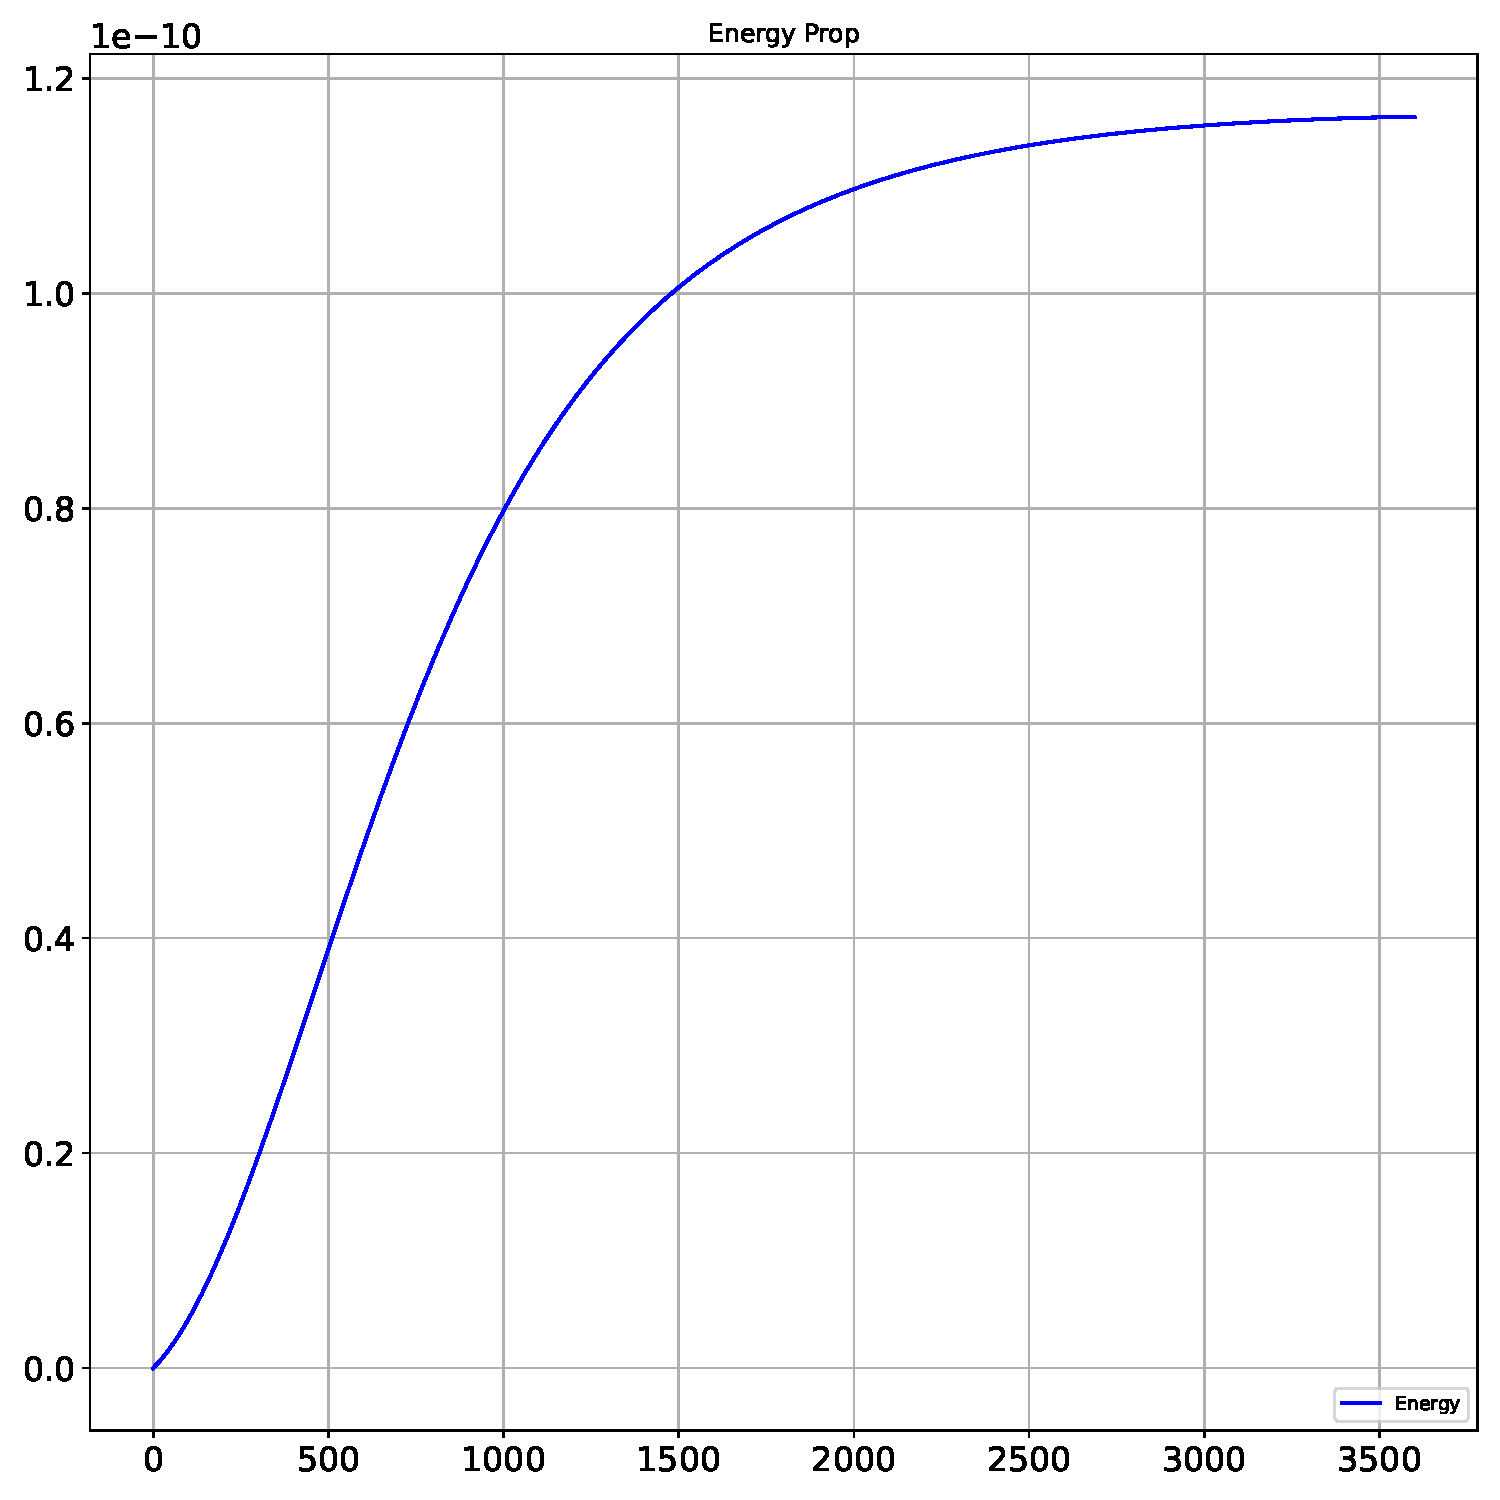
\includegraphics[height=0.9\textwidth, keepaspectratio]{AutoTeX/EnergyProp}}\caption{Orbital Energy}\label{fig:EnergyProp}\end{figure}
 \begin{figure}[htbp]\centerline{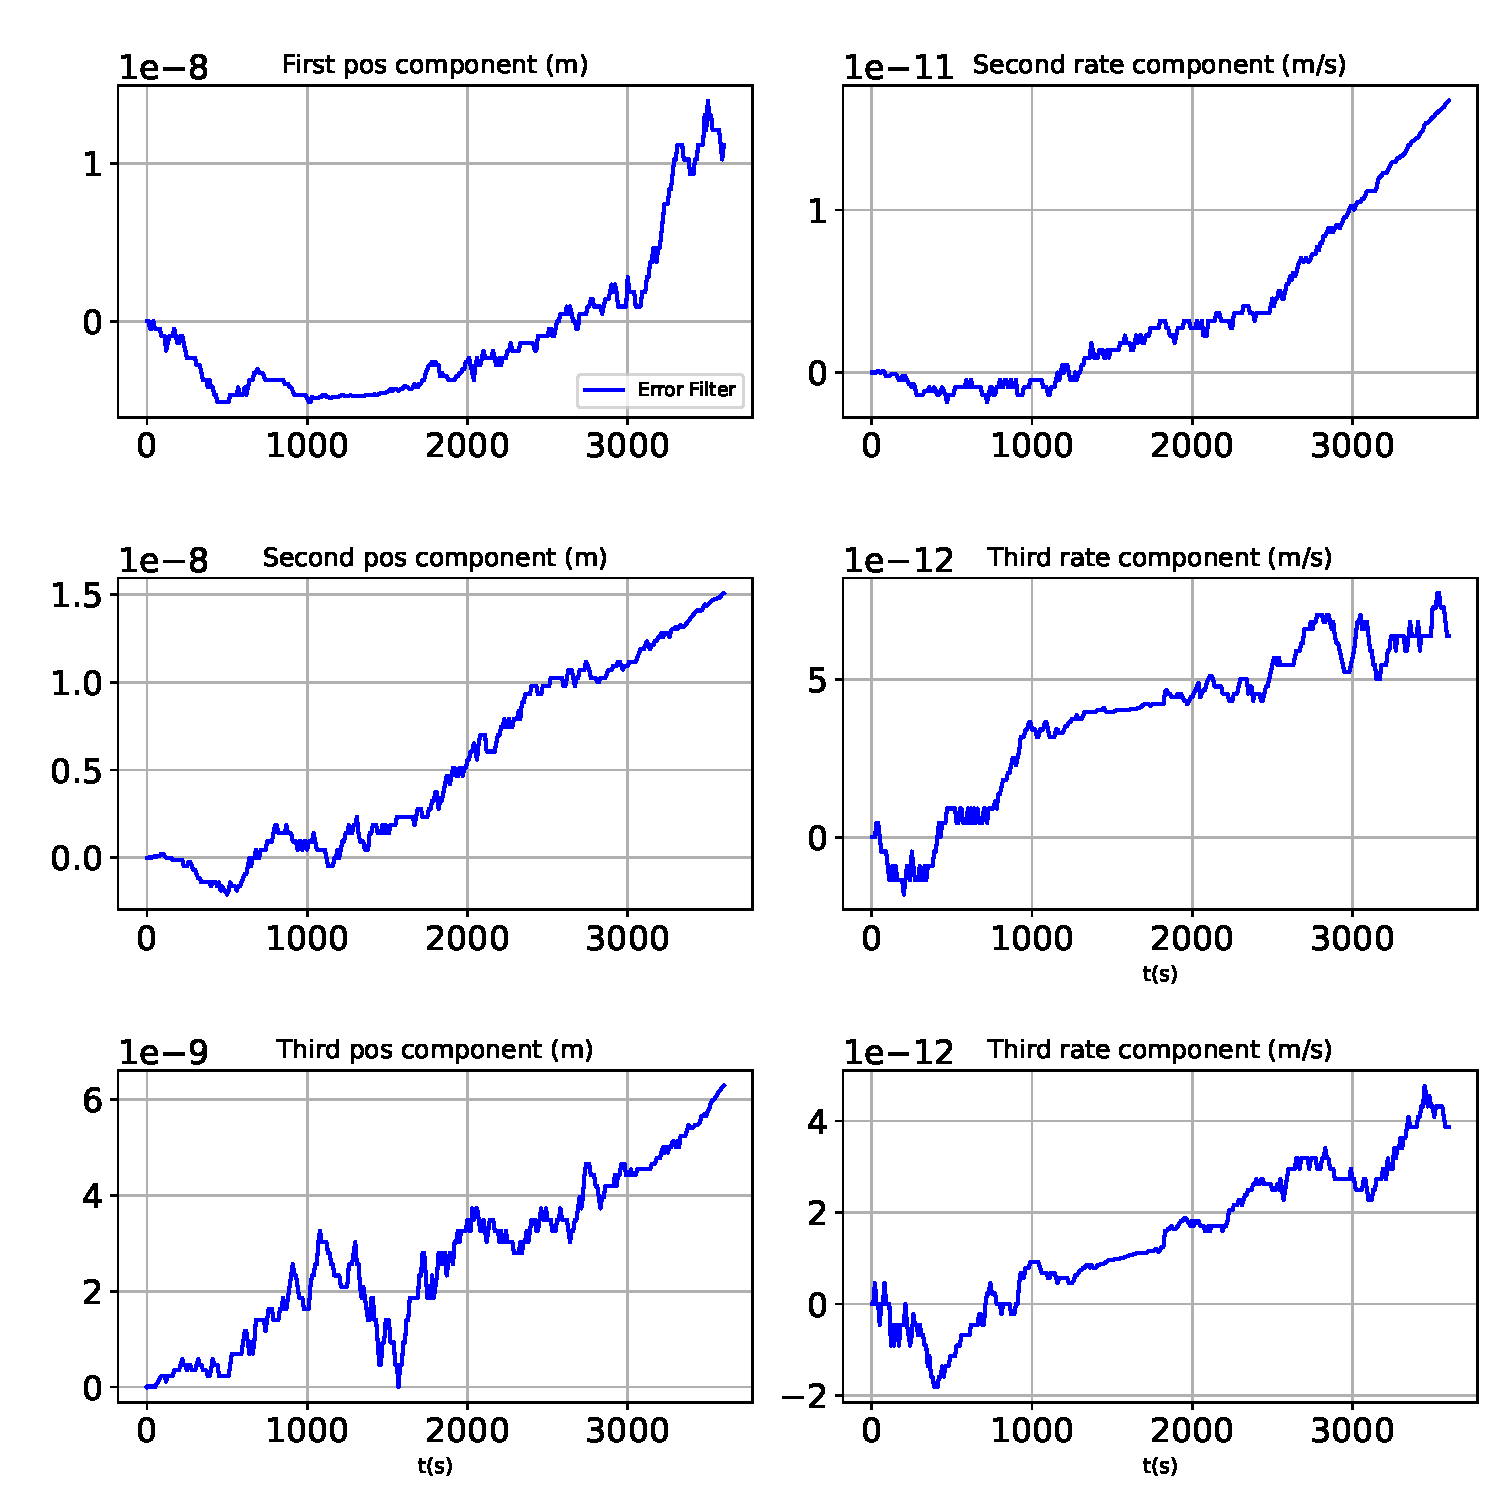
\includegraphics[height=0.9\textwidth, keepaspectratio]{AutoTeX/StatesPlotProp}}\caption{State error}\label{fig:StatesPlotProp}\end{figure}
 
Energy is conserved, and state errors are down to machine precision
 
\subsection{Test 3: State Update}

Given no unknown dynamics, this test runs the filter by giving position measurements every 50s. For the first segment of the simulation, the measurements give the expected orbit with noise. After 250s, the orbit is kicked by a velocity step and the measurement changed.

Import sim parameters are:
\begin{itemize}
\item \textbf{Timestep:} dt = 1s
\item \textbf{Planet:} Mars, $\mu = 42828.314$
\item \textbf{Noise on measurements:} $5m$
\item \textbf{Perturbation:} Velocity kick: $\left[0.,0.,0.,-0.01, 0.01, 0.02\right]$
\end{itemize}

Figures \ref{fig:EnergyUpdate} shows conservation of energy before and after the perturbation, while showing that there is indeed a unexpected event. Figure \ref{fig:StatesPlotUpdate} show the results of the state errors. It shows the rise in errors when the perturbation is introduced and how the filter resolves it. Similarly, the postfit residuals in Figure \ref{fig:PostFitUpdate} show how the filter reconverges after being kicked off track.
 \begin{figure}[htbp]\centerline{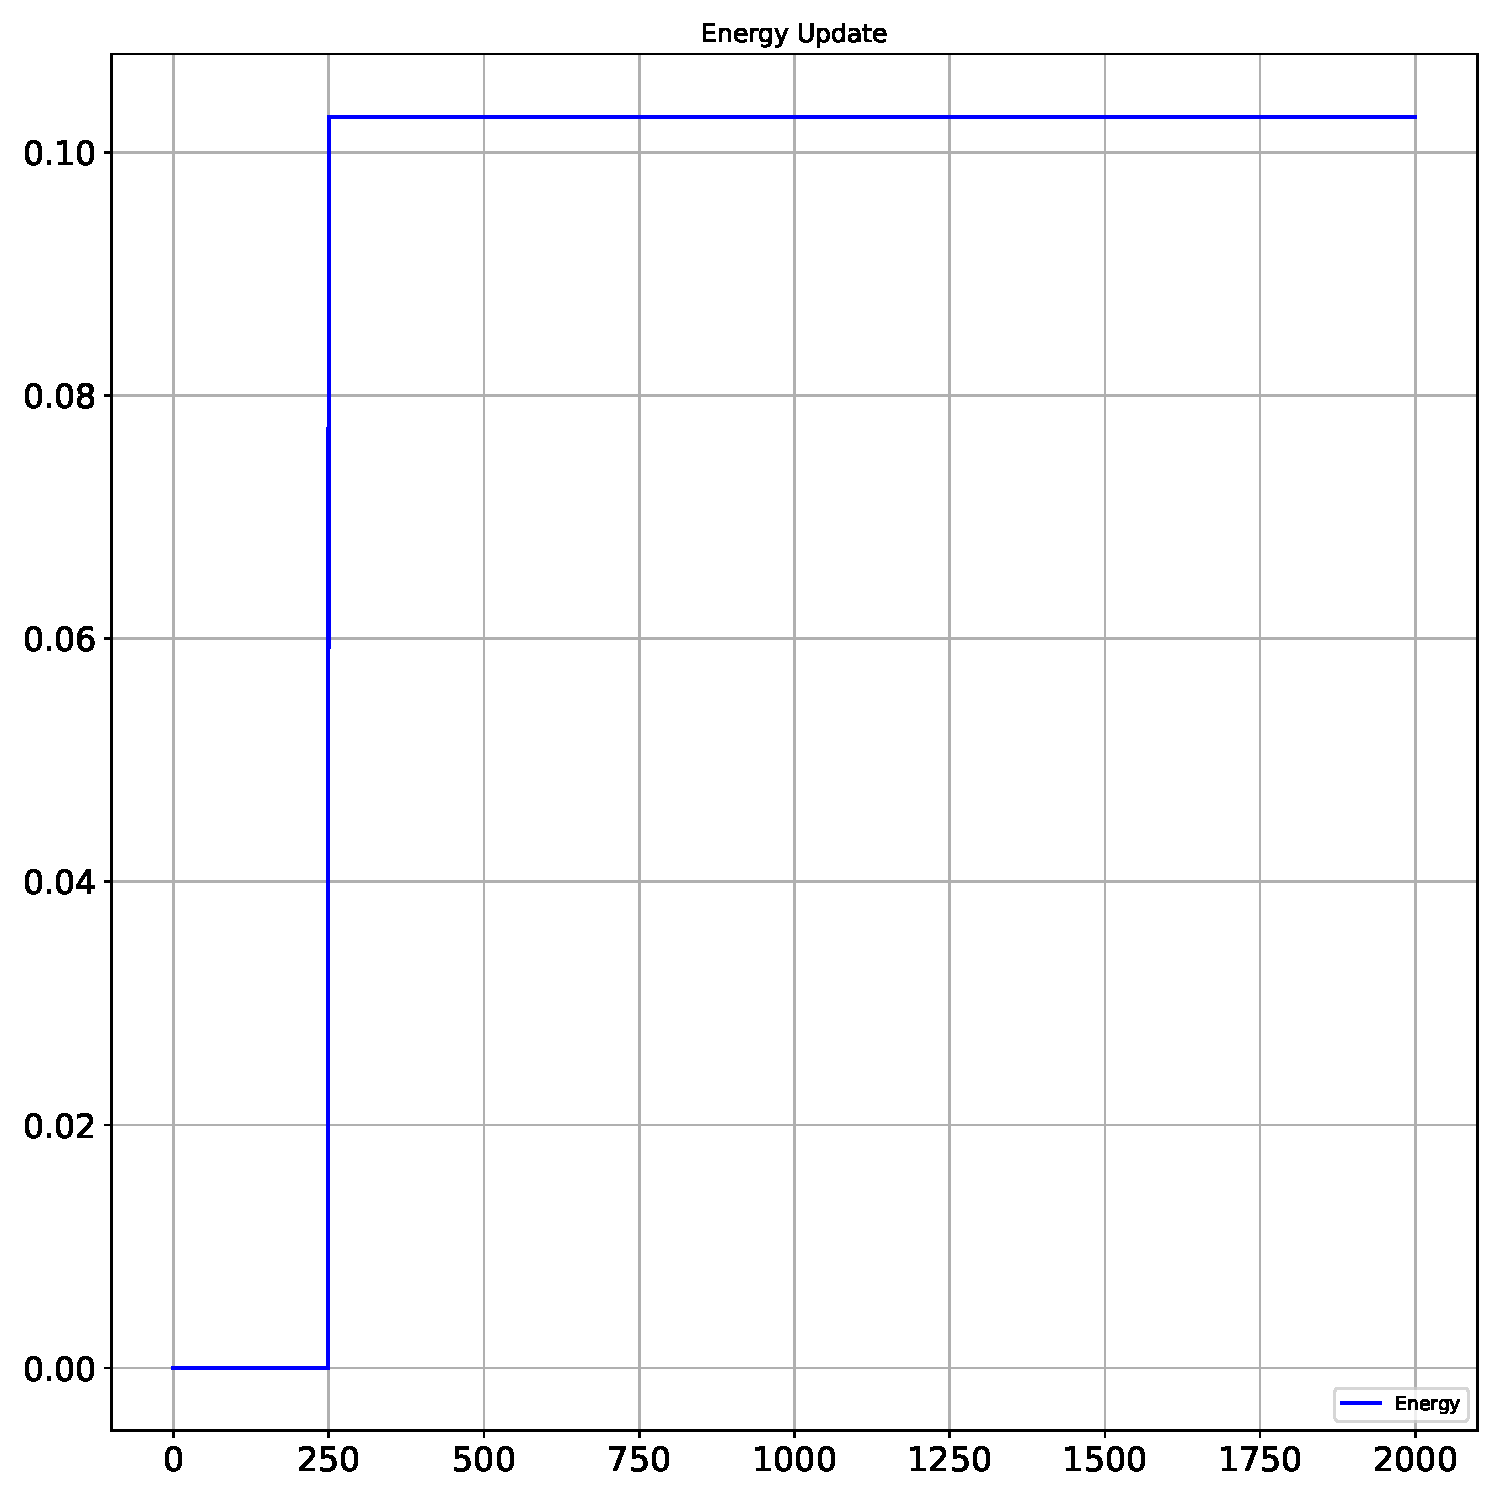
\includegraphics[height=0.9\textwidth, keepaspectratio]{AutoTeX/EnergyUpdate}}\caption{Orbital Energy}\label{fig:EnergyUpdate}\end{figure}
 \begin{figure}[htbp]\centerline{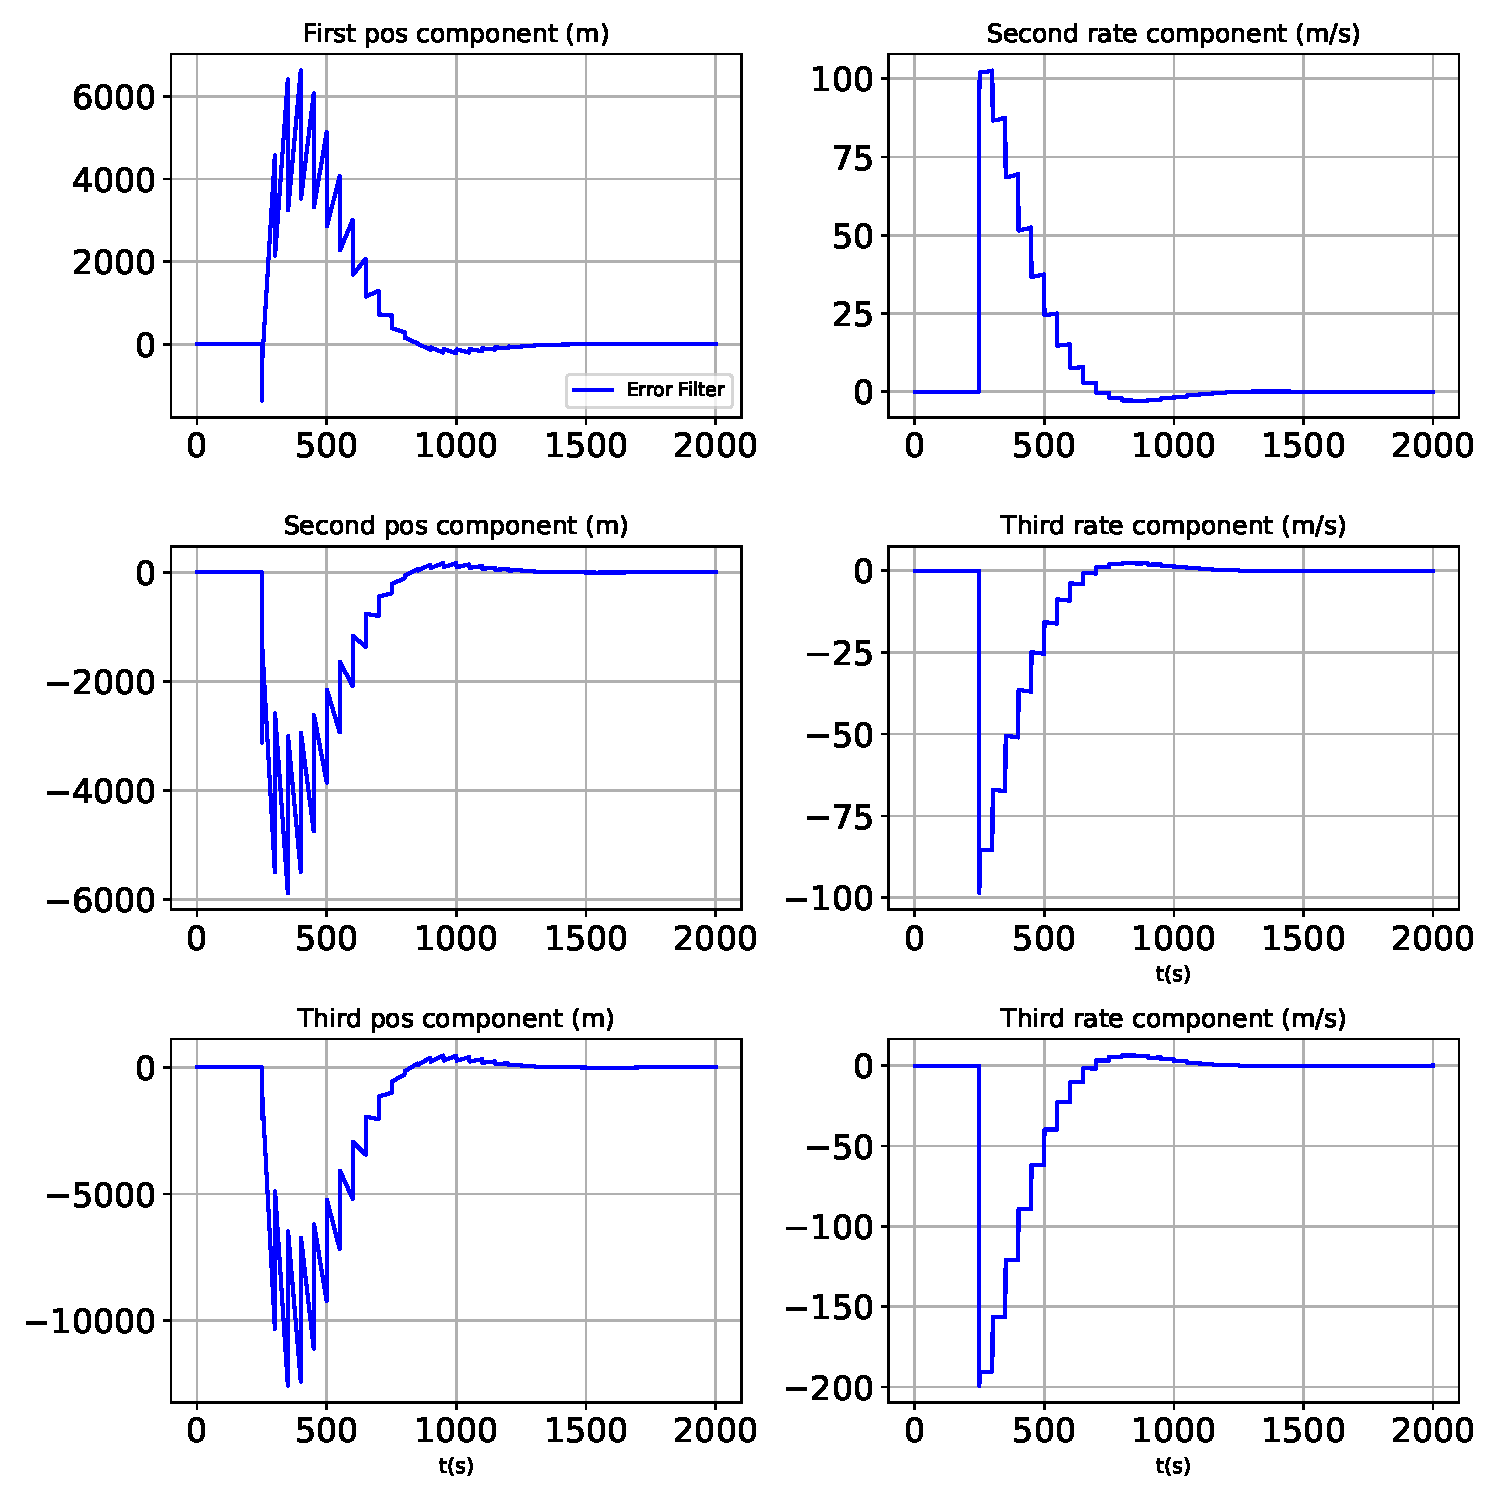
\includegraphics[height=0.9\textwidth, keepaspectratio]{AutoTeX/StatesPlotUpdate}}\caption{State error}\label{fig:StatesPlotUpdate}\end{figure}
 \begin{figure}[htbp]\centerline{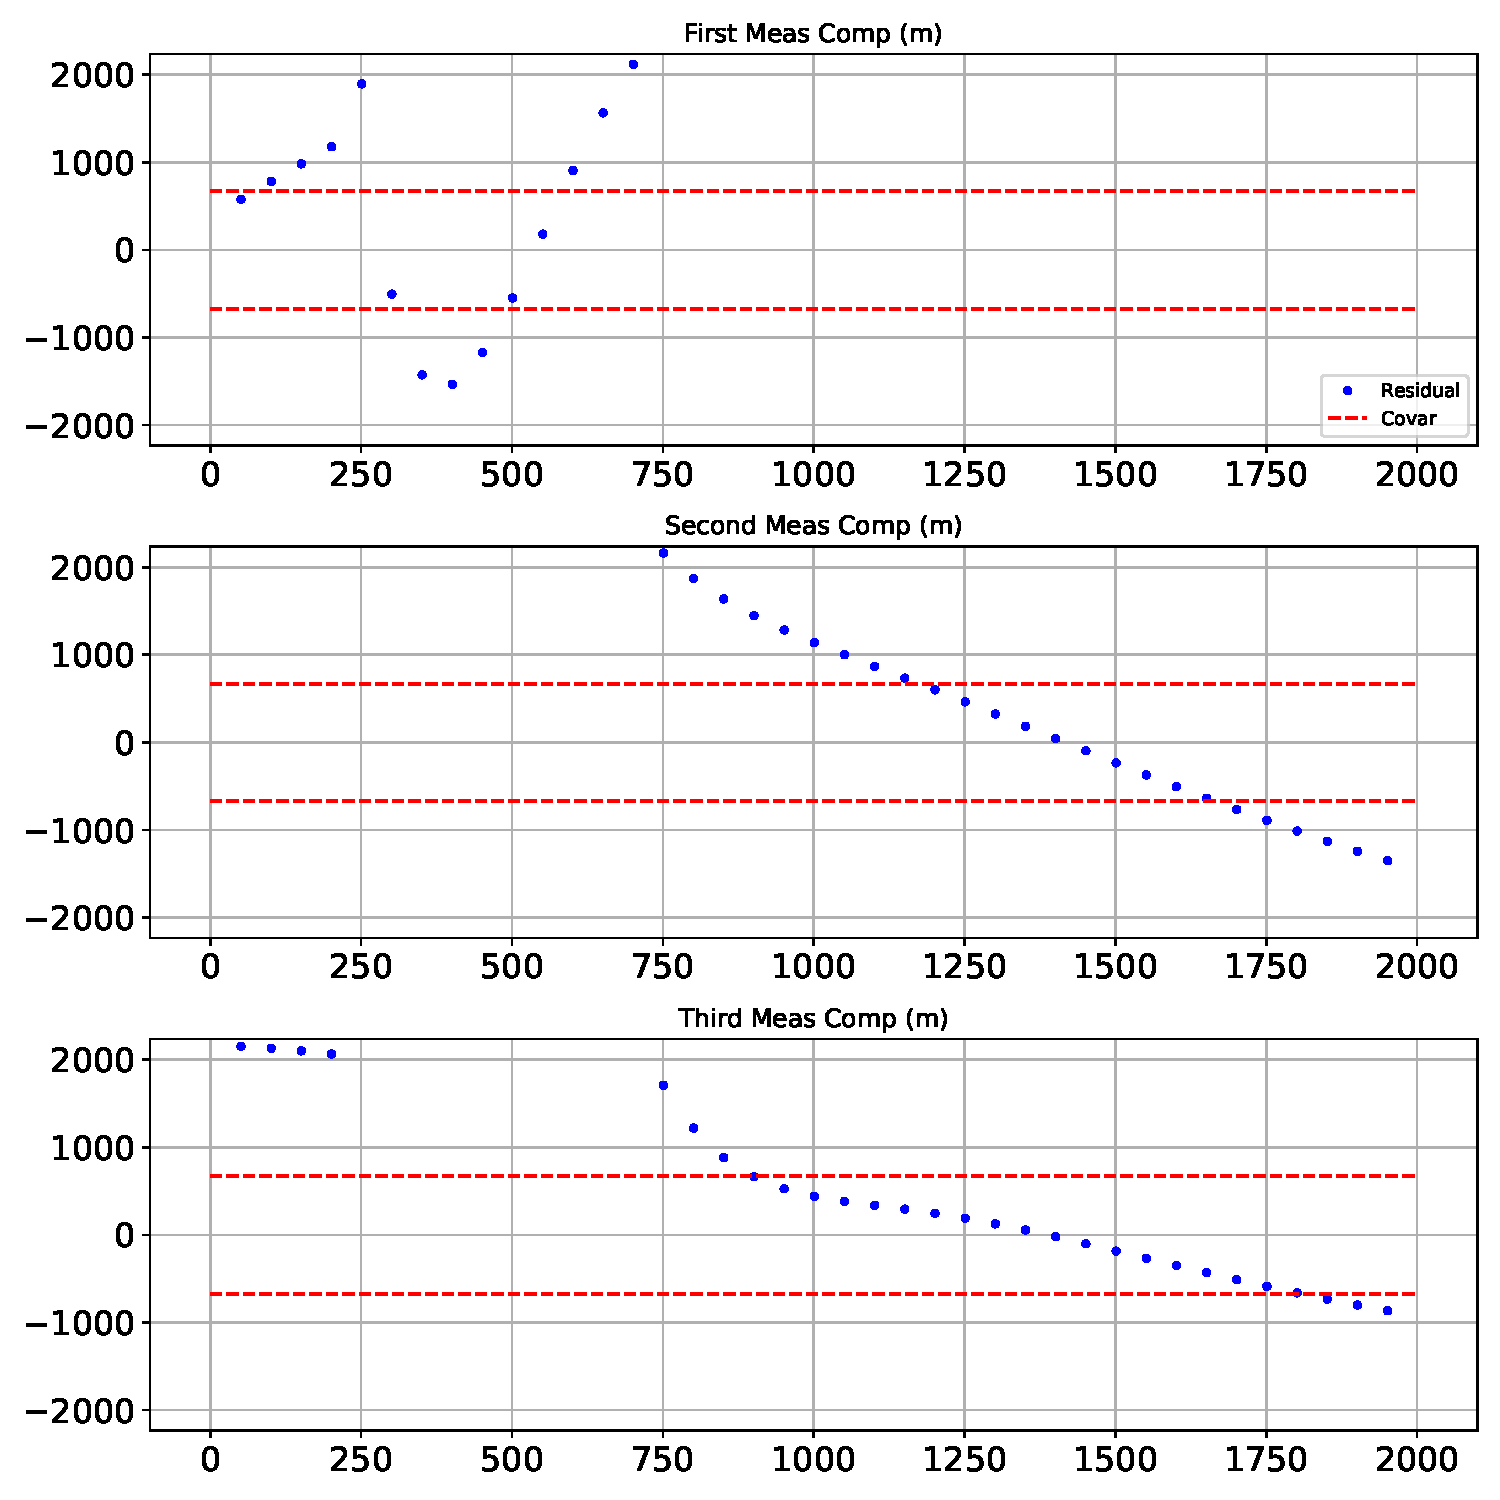
\includegraphics[height=0.9\textwidth, keepaspectratio]{AutoTeX/PostFitUpdate}}\caption{Post Fit Residuals}\label{fig:PostFitUpdate}\end{figure}
 
\section{Test Parameters}

\begin{table}[ht]
\centering
\begin{tabular}{c|c}
\hline
\hline
\textbf{Output Value Tested}     & \textbf{Tolerated Error}  \\ \hline
Test 1-Measurement 	       & 1E-15      		             \\
Test 1-Propagation	               & 1E-15     	                  \\
Test 2-Energy  	                       & 1E-10    		                   \\
Test 2-States  	                       & 1E-10    		                   \\
Test 3-Energy  	                       & 1E-10    		                   \\
Test 3-States  	                       & 1E-10    		                   \\
Test 3-Covariance  	                       & 1E-10    		                   \\		     \\\hline
\end{tabular}
\end{table}

\section{Test Results}

\begin{table}[H]
	\caption{Test results}
	\label{tab:results}
	\centering \fontsize{10}{10}\selectfont
	\begin{tabular}{c | c}
		\hline\hline
		\textbf{Check} 			&\textbf{Pass/Fail} \\ 
		\hline
	   Test 1	   			& PASS \\ 
	   Test 2	   			&PASS \\ 
	   Test 3	   			& PASS\\ 
	   \hline\hline
	\end{tabular}
\end{table}
